\section{The Euler-Lagrange Equations}
The idea is to study local behaviour of $I$ in $u\in M$, i.e. to study the function $t\longmapsto I(u+tv)$ with $t\in\mathbb{R}$ for $v\in X_0$.\\

\textbf{\underline{Definition 2.2.1}}\\
Let $u\in M$, $v\in X_0$ and $n\in\mathbb{N}$. If
\[D^nI(u)[v]:=\left.\frac{\mathrm{d}^n}{\mathrm{d}t^n}I(u+tv)\right\vert_{t=0}\]
exists, it is called the \textit{$n$-th variation of $I$ in $u$ in direction $v$}.\\[11pt]

\textbf{Remark 2.2.2}\\
The $n$-th variation is the same as the $n$-th directional derivative.\\[11pt]

\textbf{\underline{Definition 2.2.3}}\\
An element $u\in M$ is called \textit{critical point of $I$} if for all $v\in X_0$ it holds $DI(u)[v]=0$.\\[11pt]

\hypertarget{lemma_2_2_4}{\textbf{Lemma 2.2.4}}\\
(Existence of first and second variation)
\begin{itemize}
	\item[(a)] If $f\in C^1(\Omega\times\mathbb{R}^m\times\mathbb{R}^{m\times d})$ and $g\in C^1(\partial\Omega\times\mathbb{R}^m)$, then the first variation of $I$ exists and for all $u\in M$, all $v\in X_0$ we have the following
	\begin{align*}
		DI(u)[v]&=\int_\Omega{\partial_uf(x,u(x),\nabla u(x))\cdot v(x)+\partial_Af(x,u(x),\nabla u(x)):\nabla v(x)\mathrm{d}x}\\
		&\qquad\qquad+\int_{\partial\Omega}{\partial_ug(x,u(x))\cdot v(x)\mathrm{d}a}.
	\end{align*}
	\item[(b)] If $f\in C^2(\Omega\times\mathbb{R}^m\times\mathbb{R}^{m\times d})$ and $g\in C^2(\partial\Omega\times\mathbb{R}^m)$, then also the second variation of $I$ exists and for all $u\in M$, $v\in X_0$ it holds
	\begin{align*}
		D^2I(u)[v]&=\int_\Omega{D_u^2f(x,u(x),\nabla u(x))[v(x)]+2D_AD_uf(x,u(x),\nabla u(x))[v(x),\nabla v(x)]\mathrm{d}x}\\
		&\qquad\qquad+\int_\Omega{D_A^2f(x,u(x),\nabla u(x))[\nabla v(x)]\mathrm{d}x}+\int_{\partial\Omega}{D_u^2g(x,u(x))[v(x)]\mathrm{d}a}.
	\end{align*}
\end{itemize}

\textit{Remark: It would be sufficient to assume $\nabla u,\nabla v\in L^\infty(\overline{\Omega};\mathbb{R}^{m\times d})$ by Lebesgue's dominated convergence theorem.}\\

\textit{Proof:}\\
We only show the claim with the first variation, i.e. (a). The second variation works analogously. So let $u\in M$, $v\in X_0$. Then, using the main theorem of calculus in the third equation and the chain rule in the fourth,
\begin{align*}
	DI(u)[v]&=\lim_{t\to0}{\frac{1}{t}[I(u+tv)-I(u)]}\\
	&=\lim_{t\to0}{\frac{1}{t}\left[\int_\Omega{f(\cdot,u+tv,\nabla u+t\nabla v)-f(\cdot,u,\nabla u)\mathrm{d}x}+\int_{\partial\Omega}{g(\cdot,u+tv)-g(\cdot,u)\mathrm{d}a}\right]}\\
	&=\lim_{t\to0}{\frac{1}{t}\left[\int_\Omega{\int_0^1{\frac{\mathrm{d}}{\mathrm{d}\tau}f(\cdot,u+\tau tv,\nabla u+\tau t\nabla v)\mathrm{d}\tau}\mathrm{d}x}+\int_{\partial\Omega}{\int_0^1{\frac{\mathrm{d}}{\mathrm{d}\tau}g(\cdot,u+\tau tv)\mathrm{d}\tau}\mathrm{d}a}\right]}\\
	&=\lim_{t\to0}{\frac{1}{t}\left[\int_\Omega{\int_0^1{D_uf(\cdot,u+\tau tv,\nabla u+\tau t\nabla v)[tv]\mathrm{d}\tau}\mathrm{d}x}\right.}\\
	&\qquad\qquad+\int_\Omega{\int_0^1{D_Af(\cdot,u+\tau tv,\nabla u+\tau t\nabla v)[t\nabla v]\mathrm{d}\tau}\mathrm{d}x}\\
	&\qquad\qquad+\left.\int_{\partial\Omega}{\int_0^1{D_ug(\cdot,u+\tau tv)[tv]\mathrm{d}\tau}\mathrm{d}a}\right].
\end{align*}
Now the term $\frac{1}{t}$ cancels with the appearing $t$'s in the integrals coming from the directions. Since $u,v,\nabla u,\nabla v$ are bounded functions and $\partial_uf,\partial_Af,\partial_ug$ are continuous, there exists $C>0$ with
\begin{align*}
	\sup_{x\in\overline{\Omega}}{\lvert D_uf(x,u(x)+\tau tv(x),\nabla u(x)+\tau t\nabla v(x))[v(x)]\rvert}&\leq C,\\
	\sup_{x\in\overline{\Omega}}{\lvert D_Af(x,u(x)+\tau tv(x),\nabla u(x)+\tau t\nabla v(x))[\nabla v(x)]\rvert}&\leq C,\\
	\sup_{x\in\partial\Omega}{\lvert D_ug(\cdot,u(x)+\tau tv(x))[v(x)]\rvert}&\leq C.
\end{align*}
Moreover, since $f,g$ are $C^1$-functions, we have pointwise convergence of
\begin{align*}
	\lim_{t\to0}{D_uf(\cdot,u+\tau tv,\nabla u+\tau t\nabla v)[v]}&=D_uf(\cdot,u,\nabla u)[v]\\
	\lim_{t\to0}{D_Af(\cdot,u+\tau tv,\nabla u+\tau t\nabla v)[\nabla v]}&=D_Af(\cdot,u,\nabla u)[\nabla v]\\
	\lim_{t\to0}{D_ug(\cdot,u+\tau tv)[v]}&=D_ug(\cdot,u)[v].
\end{align*}
(Here, the pointwise convergence is meant in $\overline{\Omega}\times[0,1]$ and $\partial\Omega\times[0,1]$.) Lebesgue's dominated convergence theorem yields the claim.\hfill$\blacksquare$\\[11pt]

\hypertarget{theorem_2_2_5}{\textbf{\underline{Theorem 2.2.5}}}\\
(Euler-Lagrange equations)\\
Let $u\in M\cap C^2(\Omega;\mathbb{R}^m)$, $f\in C^2(\Omega\times\mathbb{R}^m\times\mathbb{R}^{m\times d})$, $g\in C^1(\partial\Omega\times\mathbb{R}^m)$. Then $u$ is a critical point of $I$ if and only if it satisfies the \textit{Euler-Lagrange equations}, i.e.
\[\text{(EL)}\qquad\left\{\begin{array}{rl}
	-\divergence{\partial_Af(\cdot,u,\nabla u)}+\partial_uf(\cdot,u,\nabla u)=0&\text{in }\Omega,\\
	u=u_0&\text{on }\Gamma_D,\\
	\partial_Af(\cdot,u,\nabla u)\cdot\nu+\partial_ug(\cdot,u)=0&\text{on }\Gamma_N.
\end{array}\right.\]

\textit{Remark: With $\nu:\partial\Omega\longrightarrow B^{d-1}\subset\mathbb{R}^d$ we denote the outer unit normal vector at $\partial\Omega$ which exists by smoothness assumption. The system (EL) is a system of $m$ coupled partial differential equations.}\\

For the proof of \hyperlink{theorem_2_2_5}{Theorem 2.2.5} we use two fundamental results.\\

\hypertarget{theorem_2_2_6}{\textbf{\underline{Theorem 2.2.6}}}\\
(Divergence Theorem by Gau{\ss})\\
Let $u\in C^1(\overline{\Omega};\mathbb{R}^m)$. Then
\[\int_\Omega{\partial_{x_j}u(x)\mathrm{d}x}=\int_{\partial \Omega}{u(x)\nu_j(x)\mathrm{d}a}\in\mathbb{R}^m.\]

\textit{Proof:}\\
This is proven in course \textit{Analysis III}.\hfill$\blacksquare$\\[11pt]

\hypertarget{theorem_2_2_7}{\textbf{\underline{Theorem 2.2.7}}}\\
(Fundamental Lemma of Calculus of Variations)\\
Let $a\in C^0(\overline{\Omega})$, $b\in C^0(\partial\Omega)$ such that
\[\int_\Omega{a(x)v(x)\mathrm{d}x}+\int_{\partial\Omega}{b(x)v(x)\mathrm{d}a}=0\]
for all $v\in C_{\Gamma_D}^\infty(\overline{\Omega})=\{v\in C^\infty(\overline{\Omega})\mid v|_{\Gamma_D}=0\}$. Then $a\equiv0$ in $\Omega$ and $b\equiv0$ on $\Gamma_N$.\\

\textit{Proof:}\\
We will prove this statement, as well as some variations of it, in the exercise class.\hfill$\blacksquare$\\[11pt]

\textit{Proof of \hyperlink{theorem_2_2_5}{Theorem 2.2.5}:}\\
For all $v\in X_0$ we have with \hyperlink{lemma_2_2_4}{Lemma 2.2.4 (a)}
\begin{align*}
	DI(u)[v]&=\int_\Omega{\partial_uf(\cdot,u,\nabla u)\cdot v+\partial_Af(\cdot,u,\nabla u):\nabla v\mathrm{d}x}+\int_{\partial\Omega}{\partial_ug(\cdot,u)\cdot v\mathrm{d}a}\\
	&=\int_\Omega{\partial_uf(\cdot,u,\nabla u)\cdot v+\divergence{v^\top\partial_Af(\cdot,u,\nabla u)}-v\cdot\divergence{\partial_Af(\cdot,u,\nabla u)}\mathrm{d}x}\\
	&\qquad\qquad+\int_{\partial\Omega}{\partial_ug(\cdot,u)\cdot v\mathrm{d}a}\\
	&=\int_\Omega{\left(\partial_uf(\cdot,u,\nabla u)-\divergence{\partial_Af(\cdot,u,\nabla u)}\right)\cdot v\mathrm{d}x}\\
	&\qquad\qquad+\int_{\partial\Omega}{\left(\partial_Af(\cdot,u,\nabla u)\cdot\nu+\partial_ug(\cdot,u)\right)\cdot v\mathrm{d}a},
\end{align*}
where we have used the divergence theorem in the last line, i.e. \hyperlink{theorem_2_2_6}{Theorem 2.2.6}. Since $u$ and $f$ are $C^2$-functions, the divergence of $\partial_Af(\cdot,u,\nabla u)$ exists. Using now the fundamental lemma of calculus of variations, \hyperlink{theorem_2_2_7}{Theorem 2.2.7}, we conclude that $DI(u)[v]=0$ for all $v\in X_0$ if and only if $u$ satisfies (EL).\hfill$\blacksquare$\\[11pt]

\textbf{Remark 2.2.8}\\
A critical point $u$ is a strong/classical solution to (EL) if $u,f$ are $C^2$-functions, but in general, $u$ is only a weak solution to (EL), that is, for all $v\in X_0$ we have
\[\int_\Omega{\partial_uf(\cdot,u,\nabla u)\cdot v+\partial_Af(\cdot,u,\nabla u):\nabla v\mathrm{d}x}+\int_{\partial\Omega}{\partial_ug(\cdot,u)\cdot v\mathrm{d}a}=0.\]\\

\textbf{Example 2.2.9}\\
(Minimal surface)\\
Let $\Omega\subset\mathbb{R}^2$ and $g\in C^0(\partial\Omega;\mathbb{R})$ be given (confer \hyperlink{example_1_2_3}{Example 1.2.3}). Find $u\in C^1(\Omega;\mathbb{R})$ with $u|_{\partial\Omega}=g$ that minimizes the area
\[I(u)=\int_\Omega{\sqrt{1+\lvert\nabla u(x)\rvert^2}\mathrm{d}x}.\]
We want to compute the Euler-Lagrange equations. In this example, $d=2$, $m=1$, $\Gamma_D=\partial\Omega$ and $\Gamma_N=\emptyset$ are our quantities. Moreover, $f(x,u,A)=\sqrt{1+\lvert A\rvert^2}$ for $A\in\mathbb{R}^2$. With that,
\[\partial_Af(x,u,A)=\frac{1}{\sqrt{1+\lvert A\rvert^2}}\begin{pmatrix}A_1\\A_2\end{pmatrix}\]
and $\partial_uf=0$. In the weak form, a critical point $u\in C^1(\Omega;\mathbb{R})$ with $u|_{\partial\Omega}=g$ satisfies
\[\int_\Omega{\frac{\nabla u(x)\cdot\nabla v(x)}{\sqrt{1+\lvert\nabla u(x)\rvert^2}}\mathrm{d}x}=0\]
for all $v\in C_0^1(\overline{\Omega})$. In the strong form, a critical point $u\in C^2(\Omega;\mathbb{R})$ with $u|_{\partial\Omega}=g$ satisfies
\[\divergence{\frac{\nabla u}{\sqrt{1+\lvert\nabla u\rvert^2}}}=0\quad\text{in }\Omega.\]
From a geometric point of view this means that the mean curvature, i.e. the sum of all principal curvatures, vanishes.\\[11pt]

\hypertarget{example_2_2_10}{\textbf{Example 2.2.10}}\\
(Heat conduction)\\
We consider an open, bounded domain $\Omega\subset\mathbb{R}^d$, a given heat source $h:\Omega\longrightarrow\mathbb{R}$ and given temperature $u_0:\Gamma_D\longrightarrow\mathbb{R}$ on a part $\Gamma_D$ of the boundary and write $u:\overline{\Omega}\longrightarrow\mathbb{R}$ for the temperature.

\begin{figure}[ht]
	\centering
	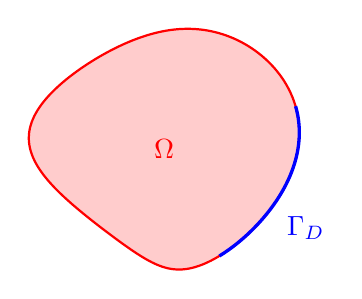
\begin{tikzpicture}
		\draw[thick, red, fill=red, fill opacity=0.2] plot[smooth, domain=0:1, samples=100] ({(1.5+0.2*cos(\x*720)+0.3*sin(\x*360))*cos(\x*360)}, {(1.5+0.3*cos(\x*360))*sin(\x*360)});
		\draw[very thick, blue] plot[smooth, domain=0.85:1.05, samples=100] ({(1.5+0.2*cos(\x*720)+0.3*sin(\x*360))*cos(\x*360)}, {(1.5+0.3*cos(\x*360))*sin(\x*360)});

		\node[red] at (0, 0) {$\Omega$};
		\node[blue] at (1.8, -1) {$\Gamma_D$};
	\end{tikzpicture}
	\caption{Example of $\Omega$ and $\Gamma_D$.}
\end{figure}

Fourier's law from physics tells that the heat flux $q$ is proportional to temperature gradient $\nabla u$. Mathematically this means there exists $K:\Omega\longrightarrow\mathbb{R}^{d\times d}$ such that $K(x)$ is symmetric, positive definite and $q(x)=-K(x)\nabla u(x)$ for each $x\in\Omega$.\\

In stationary state, it holds by physical principles
\[\int_{\partial\widetilde{\Omega}}{q(x)\cdot\nu(x)\mathrm{d}a}=\int_{\widetilde{\Omega}}{h(x)\mathrm{d}x}\]
for all $\widetilde{\Omega}\subset\Omega$. Using Gau{\ss}, this is the same as
\[\int_{\widetilde{\Omega}}{\divergence{q(x)}-h(x)\mathrm{d}x}=0\]
for $\widetilde{\Omega}\subset\Omega$, so equivalently
\[\divergence{q}-h=-\divergence{K\nabla u}-h=0\qquad\text{in }\Omega.\qquad(1)\]
If $u_\text{out}:\mathbb{R}^3\setminus\overline{\Omega}\longrightarrow\mathbb{R}$ describes the temperature outside the body, then heat exchange with
\[-(K(x)\nabla u(x))\cdot\nu(x)=q(x)\cdot\nu(x)=\alpha(x)(u(x)-u_\text{out}(x))\qquad(2)\]
for all $x\in\Gamma_N$ and some $\alpha:\partial\Omega\longrightarrow\mathbb{R}$. Then (1), (2) and $u|_{\Gamma_D}=u_0$ are the Euler-Lagrange equations of the functional
\[I(u)=\int_\Omega{\frac{1}{2}(K(x)\nabla u(x))\cdot\nabla u(x)-h(x)u(x)\mathrm{d}x}+\frac{1}{2}\int_{\partial\Omega}{\alpha(x)(u(x)-u_\text{out}(x))^2\mathrm{d}a}.\]
If we use our notations with $f$ and $g$ then this corresponds to
\begin{align*}
	f(x,u,A)&=\frac{1}{2}(K(x)A)\cdot A-h(x)u,\\
	g(x,u)&=\frac{\alpha(x)}{2}(u-u_\text{out}(x))^2.
\end{align*}
It holds $\partial_uf=-h(x)$, $\partial_Af=K(x)A$ and $\partial_ug=\alpha(x)(u-u_\text{out})$.\\[11pt]

\hypertarget{example_2_2_11}{\textbf{Example 2.2.11}}\\
(Shortest Connection)\\
Given are two points $(a,A),(b,B)\in\mathbb{R}^2$ and we want to show that the straight line is the shortest connection. Other possible connections are shown in \hyperref[fig:example_2_2_11]{Figure II.2}.\\

\begin{figure}[ht]
	\centering
	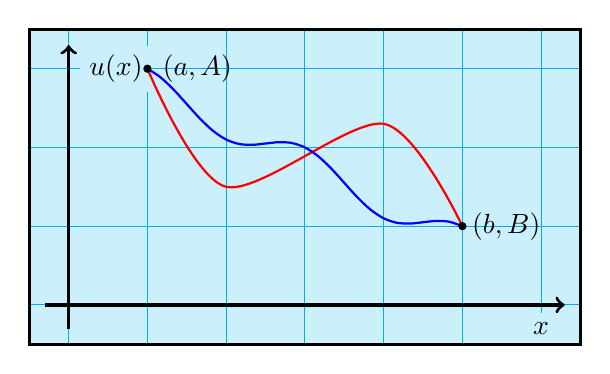
\begin{tikzpicture}
		% Hintergrund
		\fill[cyan!20] (-0.5, -0.5) rectangle (6.5, 3.5);
		\draw[thin, cyan, step=1] (-0.5, -0.5) grid (6.5, 3.5);

		% Achsen
		\draw[very thick, ->] (-0.3, 0) -- (6.3, 0);
		\draw[very thick, ->] (0, -0.3) -- (0, 3.3);
		\node[fill=cyan!20] at (6, -0.3) {$x$};
		\node[fill=cyan!20] at (0.6, 3) {$u(x)$};

		% Funktionen
		\draw[thick, red] plot[smooth] coordinates {(1, 3) (2, 1.5) (4, 2.3) (5, 1)};
		\draw[thick, blue] plot[smooth, domain=1:5] (\x, {-\x/2+0.2*cos(\x*180-180)+3.3});
		\fill (1, 3) circle (1.5pt) node[right=2] {$(a,A)$};
		\fill (5, 1) circle (1.5pt) node[right] {$(b,B)$};

		% Rahmen
		\draw[very thick] (-0.5, -0.5) rectangle (6.5, 3.5);
	\end{tikzpicture}
	\caption{Connections for $(a,A)$ and $(b,B)$.}
	\label{fig:example_2_2_11}
\end{figure}

We fix the spaces $X=C^1([a,b])$, $M=\{u\in X\mid u(a)=A,u(b)=B\}$, $X_0=C_0^1([a,b])$ and $\partial\Omega=\Gamma_D=\{a,b\}$. The length of a curve $x\mapsto(x,u(x))$ is
\[I(u)=\int_a^b{\sqrt{1+(u'(x))^2}\mathrm{d}x}\]
what we want to minimize. We have $f(x,u,A)=\sqrt{1+A^2}$ with $A\in\mathbb{R}^{1\times 1}=\mathbb{R}$ in our usual notation. With that, $\partial_uf=0$ and $\partial_Af=\frac{A}{\sqrt{1+A^2}}$. Thus, the Euler-Lagrange equation is just
\[-\frac{\mathrm{d}}{\mathrm{d}x}\left(\frac{u'}{\sqrt{1+(u')^2}}\right)=0.\]
This means $\frac{u'}{\sqrt{1+(u')^2}}=c_*$ for a constant $c_*$. Rearranging this expression leads to
\[u'(x)=\frac{c_*}{\sqrt{1-c_*^2}}\]
which is constant. So, as $u_*$ has to satisfy certain boundary conditions, we obtain
\[u_*(x)=B\frac{x-a}{b-a}+A\frac{b-x}{b-a}\]
as a possible candidate for a minimizer. Until now, we aren't able to show that this is indeed a minimizer. All what we know is that there is at most one minimizer which is $u_*$.\\[11pt]

\textbf{Remark 2.2.12}\\
By computing $u_*$ we made an observation: the quantity $\frac{u'}{\sqrt{1+(u')^2}}$ is an invariant quantity, which helped solving the (EL) equations. Invariances are an important tool to solve differential equations.\\[11pt]

\hypertarget{lemma_2_2_13}{\textbf{Lemma 2.2.13}}\\
(Special case of Noether's theorem; Emmy Noether, 1919)\\
Let
\[I(u)=\int_a^b{f(x,u(x),u'(x))\mathrm{d}x}\]
with $f\in C^2([a,b]\times\mathbb{R}^m\times\mathbb{R}^m)$.
\begin{itemize}
	\item[(a)] If $f$ does not depend on $u_k$ (with $u=(u_1,\dotsc,u_m)$), i.e. $\partial_{u_k}f=0$, then every critical point $u_*$ satisfies $\partial_{A_k}f(x,u_*(x),\nabla u_*(x))=c$ (with $A=(A_1,\dotsc,A_m)$) for all $x\in[a,b]$ for a constant $c$.
	\item[(b)] If $f$ does not depend on $x$, i.e. $\partial_xf=0$, then for every critical point $u^*\in C^2([a,b];\mathbb{R}^m)$ the function $u_*'\cdot\partial_A(u_*,u_*')-f(u_*,u_*')$ is constant in $[a,b]$.\\
\end{itemize}

\textit{Remark: In its general form, Noether's theorem says: Every continuous symmetry of variational problem on $\Omega\subset\mathbb{R}^d$ corresponds to a $d$-dimensional conservation law. If $d=1$, one obtains an invariant quantity.}\\

\textit{Proof:}
\begin{itemize}
	\item[(a)] Since $d=1$, the $k$-th component of (EL) equations reads
	\[-\left(\partial_{A_k}f(\cdot,u,\nabla u)\right)'+\partial_{u_k}f(\cdot,u,\nabla u)=0.\]
	So $\left(\partial_{A_k}f(\cdot,u,\nabla u)\right)'=0$, so $\partial_{A_k}f(\cdot,u,\nabla u)$ is constant.
	\item[(b)] Let $E(u,A)=A\cdot\partial_Af(u,A)-f(u,A)$. Then
	\begin{align*}
		\frac{\mathrm{d}}{\mathrm{d}x}(E(u_*,u_*'))&=u_*''\cdot\partial_Af(u_*,u_*')+u_*'\cdot(\partial_Af(u_*,u_*'))'\\
		&\qquad\qquad-\partial_uf(u_*,u_*')\cdot u_*'-\partial_Af(u_*,u_*')\cdot u_*''\\
		&=u_*'\cdot\left((\partial_Af(u_*,u_*'))'-\partial_uf(u_*,u_*')\right)=0
	\end{align*}
	by \hyperlink{theorem_2_2_5}{Theorem 2.2.5}.\hfill$\blacksquare$\\[11pt]
\end{itemize}

\hypertarget{example_2_2_14}{\textbf{Example 2.2.14}}\\
(Brachistochrone problem)\\
Recall the mathematical setting from \hyperlink{example_1_2_2}{Example 1.2.2}: $M=\{u\in X\mid u(a)=u_a,u(b)=u_b\}$ with $X=C^1([0,1])$, and we want to minimize
\[I(u)=\int_a^b{\sqrt{\frac{1+(u'(x))^2}{2g(u_a-u(x))}}\mathrm{d}x}.\]
The volume density is given by $f(x,u,A)=\sqrt{\frac{1+A^2}{2g(u_a-u)}}$. We see that $f$ is independent of $x$, so Noether's theorem, i.e. \hyperlink{lemma_2_2_13}{Lemma 2.2.13}, says that for critical points $u\in C^2([0,1])$ the function
\[E(u,u')=u'\cdot\frac{u'}{\sqrt{2g(u_a-u)(1+(u')^2)}}-\sqrt{\frac{1+(u')^2}{2g(u_a-u)}}=\frac{-1}{\sqrt{2g(u_a-u)(1+(u')^2)}}\]
is constant in $x$. Hence, $(1+(u')^2)(u_a-u)=c$ for some $c>0$. This leads to
\[u'=\pm\sqrt{\frac{c}{u_a-u}-1}=:h(u),\]
so
\[\int_{u_a}^u{\frac{\mathrm{d}v}{h(v)}}=x+a.\]
This is an elliptic integral from which one can obtain an implicit formula for $u$. (To be precise, one needs to argue a little bit more because $h$ could be zero. However, $h$ cannot be zero on an interval $(a,x_0)$ because we then would have $I(u)=+\infty$. Hence, we obtain at least a local solution which can be extended to a global solution.)\\[11pt]

\textbf{Example 2.2.15}\\
(Minimal surface of revolution)\\
Recall from \hyperlink{example_1_2_3}{Example 1.2.3 (b)} that we want to minimize the functional
\[I(u)=\int_0^L{2\pi u(x)\sqrt{1+(u'(x))^2}\mathrm{d}x}\]
on $M=\{u\in C^1([0,L])\mid u(0)=u_0,u(L)=u_L\}$ for given $L,u_0,u_L>0$. The volume density is $f(x,u,A)=2\pi u\sqrt{1+A^2}$, and the derivatives are given by $\partial_uf(x,u,A)=2\pi\sqrt{1+A^2}$, $\partial_Af(x,u,A)=\frac{2\pi uA}{\sqrt{1+A^2}}$. Assume $u\in C^2([0,L])\cap M$ is a critical point. Then $u$ satisfies the Euler-Lagrange equations, which here is just the equation
\[-\left(\frac{2\pi uu'}{\sqrt{1+(u')^2}}\right)'+2\pi\sqrt{1+(u')^2}=0.\]
However, this is a scalar equation of second order and not so easy to solve. Observe that $f$ is independent of $x$. Thus, Noether's theorem tells us (after division by $2\pi$)
\[c=u\frac{(u')^2}{\sqrt{1+(u')^2}}-u\sqrt{1+(u')^2}=\frac{-u}{\sqrt{1+(u')^2}}\]
for some $c\in\mathbb{R}$. This transforms to $1+(u')^2=u^2c^{-2}$, i.e.
\[u'=\pm\sqrt{\frac{u^2}{c^2}-1}.\]
Note that $u$ cannot be constant in $[0,L]$ because then it would be no longer a solution for the Euler-Lagrange equation in general. So for some $x_0\in[0,L)$, the solution must be given in the form
\[u(x)=c\cdot\cosh\left(\frac{x-d}{c}\right)\]
on $(x_0,L)$ and constant in $(0,x_0)$ (via integration like in \hyperlink{example_2_2_14}{Example 2.2.14}). But since $u$ is twice continuously differentiable it must hold
\[u''(x_0)=\frac{1}{c}\cosh\left(\frac{x_0-d}{c}\right)>0,\]
and if $x_0>0$ then also $u''(x_0)=0$ which is a contradiction, so $x_0=0$. Determine $c,d\in\mathbb{R}$ by $u(0)=u_0$ and $u(b)=u_L$.